\documentclass[10pt,UTF8]{ctexart}


\usepackage[margin=2cm,a4paper]{geometry}
%\usepackage[left=0.75in,top=0.6in,right=0.75in,bottom=1.0in,a4paper]{geometry}

\setmainfont{Caladea}
%% 也可以選用其它字庫:
% \setCJKmainfont[%
%   ItalicFont=AR PL KaitiM GB,
%   BoldFont=Noto Sans CJK SC,
% ]{Noto Serif CJK SC}
% setCJKsansfont{Noto Sans CJK SC}
% \renewcommand{\kaishu}{\CJKfontspec{AR PL KaitiM GB}}

% 繁體中文
\setCJKmainfont[Path=fonts/ ]{NotoSansTC-Medium.otf}

\usepackage{minted}
\usepackage[breaklinks]{hyperref}

% Picture
% 導言區的此三行無變化
\usepackage{graphicx}
\usepackage{float} 
\usepackage{subfigure}
% 以下是新增的自定義格式更改
\usepackage[]{caption2} %新增調用的宏包
\renewcommand{\figurename}{Fig.} %重定義編號前綴詞
\renewcommand{\captionlabeldelim}{.~} %重定義分隔符
 %\roman 是羅馬數字編號,\alph是默認的字母編號,\arabic是阿拉伯數字編號,可按需替換下一行的相應位置
\renewcommand{\thesubfigure}{(\roman{subfigure})}%此外,還可設置圖編號顯示格式,加括號或者不加括號
\makeatletter \renewcommand{\@thesubfigure}{\thesubfigure \space}%子圖編號與名稱的間隔設置
\renewcommand{\p@subfigure}{} \makeatother

% Math
\usepackage {mathtools}
\usepackage{amssymb}

% Code
\usepackage{listings}
\usepackage{xcolor}
\lstset{
    % backgroundcolor=\color{red!50!green!50!blue!50},
    % 程式碼塊背景色為淺灰色
    rulesepcolor= \color{gray}, % 程式碼塊邊框顏色
    breaklines=true,  % 程式碼過長則換行
    numbers=left, % 行號在左側顯示
    numberstyle= \small,% 行號字型
    % eywordstyle= \color{red,% 關鍵字顏色
    commentstyle=\color{gray}, % 註釋顏色
    frame=shadowbox % 用方框框住程式碼塊
    }

\usepackage{hyperref}

\title{算法分析和複雜性理論}
\author{干皓丞,2101212850, 信息工程學院}

\begin{document}
\maketitle


\section{作業目標與章節摘要}

1. LeetCode 743. Network Delay Time 網絡延遲時間

2. LeetCode 847. Shortest Path Visiting All Nodes 訪問所有節點的最短路徑


\section{作業內容概述}

作業可以從 GitHub 下的 kancheng/kan-cs-report-in-2022 專案找到,作業程式碼與文件目錄為 kan-cs-report-in-2022/AATCC/lab-report/。實際執行的環境與實驗設備為 Google 的 Colab 、MacBook Pro (Retina, 15-inch, Mid 2014) 、 Acer Aspire R7 與 HP Victus (Nvidia GeForce RTX 3060)。

本作業 GitHub 專案為 kancheng/kan-cs-report-in-2022 下的 AATCC` 的目錄。程式碼可以從 code 目錄下可以找到 *.pynb,內容包含上次課堂練習、LeetCode 範例思路整理與作業。

https://github.com/kancheng/kan-cs-report-in-2022/tree/main/AATCC

\begin{figure}[H]
\centering 

\includegraphics[width=0.30\textwidth]{aatccqr.png} 
\caption{作業專案位置}
\label{Test}
\end{figure}


1. LeetCode : https://leetcode.com/

2. LeetCode CN : https://leetcode-cn.com/

3. OnlineGDB : https://www.onlinegdb.com/ 

LeetCode 的平台部分, CN 的平台有針對簡體中文使用者進行處理,包含中英文切換等功能。OnlineGDB 則可線上進行簡易的環境測試,其程式碼涵蓋 C, C++, C\#, Java, Python, JS, Rust, Go。

\newpage

\section{LeetCode 743. Network Delay Time 網絡延遲時間}

\subsection{LeetCode 743. 題目}

You are given a network of n nodes, labeled from 1 to n. You are also given times, a list of travel times as directed edges times[i] = (ui, vi, wi), where ui is the source node, vi is the target node, and wi is the time it takes for a signal to travel from source to target.

We will send a signal from a given node k. Return the minimum time it takes for all the n nodes to receive the signal. If it is impossible for all the n nodes to receive the signal, return -1.

有 n 個網絡節點,標記為 1 到 n。給你一個列表 times,表示信號經過 有向 邊的傳遞時間。 times[i] = (ui, vi, wi),其中 ui 是源節點,vi 是目標節點, wi 是一個信號從源節點傳遞到目標節點的時間。現在,從某個節點 K 發出一個信號。需要多久才能使所有節點都收到信號?如果不能使所有節點收到信號,返回 -1 。

\begin{figure}[H]
\centering 
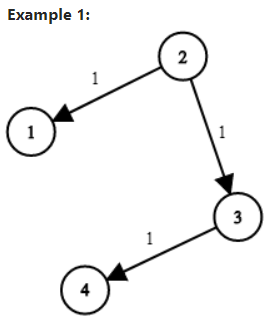
\includegraphics[width=0.40\textwidth]{lc-743-p-example.png} 
\caption{Example}
\label{Test}
\end{figure}

Example 1:

\begin{lstlisting}[language={python}]
Input: times = [[2,1,1],[2,3,1],[3,4,1]], n = 4, k = 2
Output: 2
\end{lstlisting}

Example 2:

\begin{lstlisting}[language={python}]
Input: times = [[1,2,1]], n = 2, k = 1
Output: 1
\end{lstlisting}

Example 3:

\begin{lstlisting}[language={python}]
Input: times = [[1,2,1]], n = 2, k = 2
Output: -1
\end{lstlisting}

Constraints:

1. 1 <= k <= n <= 100

2. 1 <= times.length <= 6000

3. times[i].length == 3

4. 1 <= ui, vi <= n

5. ui != vi

6. 0 <= wi <= 100

7. All the pairs (ui, vi) are unique. (i.e., no multiple edges.)

8. 所有 (ui, vi) 對都 互不相同(即,不含重複邊)


\subsection{LeetCode 743. 思路總結}

計算源點到其他所有點所需的時間,記錄在數組 dist[]中,返回 dist[]中的最大值,即延遲時間

\subsection{LeetCode 743. Code 範例}

\begin{lstlisting}[language={python}]
from typing import List
class Solution:
    # Bellman-Ford 算法
    def networkDelayTime(self, times: List[List[int]], n: int, k: int) -> int:
        dis={node:float('inf') for node in range(1,n+1)}
        dis[k]=0
        for _ in range(n-1):
            for u,v,w in times:
                dis[v]=min(dis[v],dis[u]+w)
        res=max(dis.values())
        return res if res != float('inf') else -1   
\end{lstlisting}

\subsection{LeetCode 743. 結果}

\begin{figure}[H]
\centering 
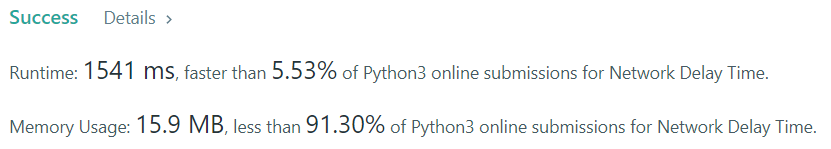
\includegraphics[width=0.80\textwidth]{lc-743-o.png} 
\caption{LeetCode 743. 結果}
\label{Test}
\end{figure}


\newpage

\section{LeetCode 847. Shortest Path Visiting All Nodes 訪問所有節點的最短路徑}

\subsection{LeetCode 847. 題目}

You have an undirected, connected graph of n nodes labeled from 0 to n - 1. You are given an array graph where graph[i] is a list of all the nodes connected with node i by an edge.

Return the length of the shortest path that visits every node. You may start and stop at any node, you may revisit nodes multiple times, and you may reuse edges.

存在一個由 n 個節點組成的無向連通圖,圖中的節點按從 0 到 n - 1 編號。

給你一個數組 graph 表示這個圖。其中,graph[i] 是一個列表,由所有與節點 i 直接相連的節點組成。

返回能夠訪問所有節點的最短路徑的長度。你可以在任一節點開始和停止,也可以多次重訪節點,並且可以重用邊。

\begin{figure}[H]
\centering 
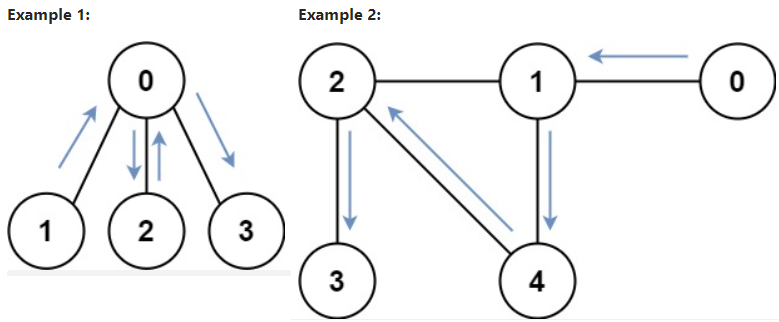
\includegraphics[width=0.80\textwidth]{lc-847-p-example.png} 
\caption{Example}
\label{Test}
\end{figure}

Example 1:

\begin{lstlisting}[language={python}]
Input: graph = [[1,2,3],[0],[0],[0]]
Output: 4
Explanation: One possible path is [1,0,2,0,3]
一種可能的路徑為 [1,0,2,0,3]
\end{lstlisting}

Example 2:

\begin{lstlisting}[language={python}]
Input: graph = [[1],[0,2,4],[1,3,4],[2],[1,2]]
Output: 4
Explanation: One possible path is [0,1,4,2,3]
一種可能的路徑為 [0,1,4,2,3]
\end{lstlisting}

Constraints:

1. n == graph.length

2. 1 <= n <= 12

3. 0 <= graph[i].length < n

4. graph[i] does not contain i.(graph[i] 不包含 i)

5. If graph[a] contains b, then graph[b] contains a.(如果 graph[a] 包含 b ,那麼 graph[b] 也包含 a)

6. The input graph is always connected.(輸入的圖總是連通圖)

\subsection{LeetCode 847. 思路總結}

本题中节点数量 n <= 12,因此可结合二进制方法进行状态压缩。设计一个动态规划数组 dp, 其中 dp[j][i] 表示节点访问状态为 i (即 i 二进制位为 1 对应的节点已被访问),且当前节点为 j 时的最短路径长度。则状态转移方程为:

dp[j][i] = Math.min(dp[j][i], dp[k][i \^ (1 << j)] + dis[k][j]),其中 k 为可能的上一节点,dis[k][j] 表示节点 k 和 j 间的距离。
因为计算过程中 dis[i][j] 会被多次使用,可结合 floyd 算法,先预处理计算得到任意 2 点间的距离。

\subsection{LeetCode 847. Code 範例}

\begin{lstlisting}[language={python}]
class Solution:
    def shortestPathLength(self, graph: List[List[int]]) -> int:
        q = collections.deque([])
        visited = set()
        n = len(graph)
        for i in range(n):
            q.append((i, 1 << i))
            visited.add((i, 1 << i))
        dis = 0
        while q:
            dis += 1
            for _ in range(len(q)):
                cur, cur_state = q.popleft()
                for nxt in graph[cur]:
                    nxt_state = cur_state | (1 << nxt)
                    if nxt_state == (1 << n) - 1: return dis
                    if (nxt, nxt_state) not in visited:
                        q.append((nxt, nxt_state))
                        visited.add((nxt, nxt_state))
        return 0
\end{lstlisting}

\subsection{LeetCode 847. 結果}

\begin{figure}[H]
\centering 
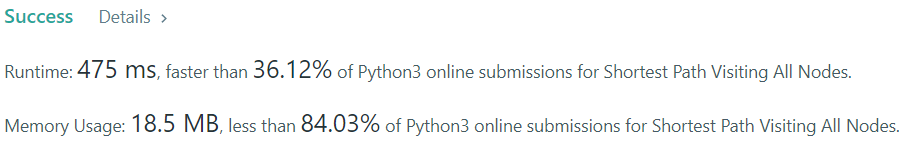
\includegraphics[width=0.80\textwidth]{lc-847-o.png} 
\caption{LeetCode 847. 結果}
\label{Test}
\end{figure}





%\section{附錄}

% 數學意義說明

% $$\min \limits_{G}\max \limits_{D}{V_I(D,\ G)=V(D,G)-\lambda L_I(G,Q)}$$

%	\begin{lstlisting}[language={python}]

%	\end{lstlisting}

%\begin{enumerate}
%\item Y
%\item A
%\end{enumerate}

% \newpage

\clearpage

\end{document}